\PassOptionsToPackage{table}{xcolor}
\documentclass[aspectratio=169,10pt]{beamer}

\usepackage[T1]{fontenc}
\usepackage[utf8]{inputenc}
\usepackage{lmodern}
\usepackage{amsmath}
\usepackage{amssymb}
\usepackage{tikz}
\usetikzlibrary{positioning, calc, shapes.geometric, arrows.meta, backgrounds}
\usepackage{tcolorbox}
\tcbuselibrary{skins}
\usepackage{booktabs}
\usepackage{colortbl}
\usepackage[ruled,vlined,linesnumbered]{algorithm2e}
\usepackage{listings}
\usepackage{fontawesome5}
\usepackage{array}

% ---------------------------------------------------------------------------
% Palette
% ---------------------------------------------------------------------------
\definecolor{navyDeep}{RGB}{20,33,61}
\definecolor{navySoft}{RGB}{36,52,84}
\definecolor{tealAccent}{RGB}{0,168,150}
\definecolor{amberAccent}{RGB}{255,159,28}
\definecolor{paperGray}{RGB}{246,247,249}
\definecolor{inkGray}{RGB}{90,98,110}

\setbeamercolor{normal text}{fg=navyDeep, bg=white}
\setbeamercolor{structure}{fg=tealAccent}
\setbeamercolor{alerted text}{fg=amberAccent}
\setbeamercolor{title}{fg=navyDeep}
\setbeamercolor{frametitle}{bg=navyDeep, fg=white}
\setbeamercolor{footlinelight}{bg=paperGray, fg=inkGray}
\setbeamercolor{footlinedark}{bg=navyDeep, fg=white}
\setbeamercolor{block title}{bg=navySoft, fg=white}
\setbeamercolor{block body}{bg=paperGray, fg=navyDeep}
\setbeamercolor{itemize item}{fg=tealAccent}
\setbeamercolor{itemize subitem}{fg=amberAccent}
\setbeamercolor{section in toc}{fg=navyDeep}
\setbeamercolor{caption name}{fg=tealAccent}

\setbeamerfont{frametitle}{series=\bfseries, size=\large}
\setbeamerfont{footline}{size=\tiny}
\setbeamertemplate{navigation symbols}{}
\setbeamertemplate{itemize item}{\faAngleRight}
\setbeamertemplate{itemize subitem}{\faCircle[regular]}

\setbeamertemplate{frametitle}{%
  \vspace{0.1em}%
  \hspace{-1em}%
  \begin{beamercolorbox}[wd=\paperwidth,ht=3.4em,dp=0.6em,leftskip=1.2em]{frametitle}
    {\insertframetitle}\\[-0.1em]
    {\small\normalfont\color{amberAccent}\insertframesubtitle}
  \end{beamercolorbox}%
}

\setbeamertemplate{footline}{%
  \leavevmode
  \hbox{%
  \begin{beamercolorbox}[wd=.72\paperwidth,ht=2.6ex,dp=1ex,left,leftskip=1em]{footlinelight}
    \usebeamerfont{footline}\textsc{Nimbus Stream Walkthrough}\hspace{0.6em}\textbullet\hspace{0.6em}Synapse Platform Team
  \end{beamercolorbox}%
  \begin{beamercolorbox}[wd=.28\paperwidth,ht=2.6ex,dp=1ex,right,rightskip=1em]{footlinedark}
    \usebeamerfont{footline}\insertframenumber{} / \inserttotalframenumber
  \end{beamercolorbox}}%
}

% ---------------------------------------------------------------------------
% Code listing style
% ---------------------------------------------------------------------------
\lstdefinestyle{nimbus}{
  basicstyle=\ttfamily\scriptsize\color{navyDeep},
  keywordstyle=\bfseries\color{tealAccent},
  commentstyle=\itshape\color{inkGray},
  stringstyle=\color{amberAccent},
  numbers=left,
  numberstyle=\tiny\color{inkGray},
  numbersep=6pt,
  backgroundcolor=\color{paperGray},
  frame=single,
  rulecolor=\color{navySoft},
  framerule=0.6pt,
  breaklines=true,
  showstringspaces=false,
  tabsize=2,
  morekeywords={func,if,else,return,for,range,go,select,case,var,struct,map,chan,defer}
}

% ---------------------------------------------------------------------------
% Stat callout box
% ---------------------------------------------------------------------------
\newtcolorbox{statbox}[1]{%
  colback=white, colframe=tealAccent, boxrule=0.8pt, arc=2pt,
  left=6pt, right=6pt, top=5pt, bottom=5pt,
  title={#1}, coltitle=white, colbacktitle=navySoft,
  fonttitle=\bfseries\small, boxsep=1pt
}

% ---------------------------------------------------------------------------
% Section divider frame
% ---------------------------------------------------------------------------
\newcommand{\sectiondivider}[2]{%
\begingroup
\setbeamercolor{background canvas}{bg=navyDeep}
\begin{frame}[plain]
  \begin{tikzpicture}[remember picture, overlay]
    \fill[amberAccent] (current page.south west) rectangle ($(current page.south east)+(0,0.12)$);
    \fill[tealAccent] ($(current page.north west)-(0,0.12)$) rectangle (current page.north east);
  \end{tikzpicture}
  \vfill
  \centering
  {\usebeamerfont{title}\color{white}\Huge\bfseries #1\par}
  \vspace{0.6em}
  {\color{tealAccent}\large #2\par}
  \vfill
\end{frame}
\endgroup
}

\title[Nimbus Stream Walkthrough]{Building Nimbus Stream}
\subtitle{A Technical Walkthrough of Synapse's Real-Time Event Pipeline}
\author{Maya Chen \\ \small Staff Engineer, Platform Team}
\institute{Synapse}
\date{Engineering All-Hands \textbullet\ July 2026}

\begin{document}

% ---------------------------------------------------------------------------
\begin{frame}[plain]
  \begin{tikzpicture}[remember picture, overlay]
    \fill[navyDeep] (current page.south west) rectangle (current page.north east);
    \fill[tealAccent] (current page.south west) rectangle ($(current page.south east)+(0,0.14)$);
    \fill[amberAccent] ($(current page.north west)-(0,0.14)$) rectangle (current page.north east);
    \node[anchor=south east, xshift=-0.6cm, yshift=0.9cm] at (current page.south east) {%
      \begin{tikzpicture}
        \foreach \i/\c in {0/tealAccent,1/amberAccent,2/tealAccent}{
          \node[circle, draw=\c, fill=\c!20, minimum size=0.5cm] at (\i*0.55,0) {};
        }
      \end{tikzpicture}%
    };
  \end{tikzpicture}
  \vspace{1.2cm}
  \centering
  {\color{tealAccent}\normalsize\textsc{Synapse Platform Team}\par}
  \vspace{0.4em}
  {\color{white}\Huge\bfseries Building Nimbus Stream\par}
  \vspace{0.3em}
  {\color{white!85!black}\Large A Technical Walkthrough of Synapse's\\ Real-Time Event Pipeline\par}
  \vspace{1.4em}
  {\color{amberAccent}\rule{4cm}{0.8pt}\par}
  \vspace{1.0em}
  {\color{white}\large Maya Chen\par}
  {\color{tealAccent}\small Staff Engineer, Platform Team\par}
  \vspace{0.8em}
  {\color{white!70!black}\small Engineering All-Hands \textbullet\ July 2026\par}
\end{frame}

% ---------------------------------------------------------------------------
\begin{frame}{Agenda}{What we'll cover in the next 25 minutes}
  \begin{columns}[T,onlytextwidth]
    \begin{column}{0.5\textwidth}
      \begin{enumerate}
        \setbeamertemplate{enumerate item}{\color{tealAccent}\bfseries\insertenumlabel}
        \item Problem \& context
        \item System architecture
        \item Core algorithm: adaptive partitioning
      \end{enumerate}
    \end{column}
    \begin{column}{0.5\textwidth}
      \begin{enumerate}
        \setbeamertemplate{enumerate item}{\color{tealAccent}\bfseries\arabic{enumi}}
        \setcounter{enumi}{3}
        \item Results \& benchmarks
        \item Lessons learned
      \end{enumerate}
    \end{column}
  \end{columns}
  \vspace{0.8em}
  \begin{statbox}{Why this matters}
    Nimbus Stream now routes \textbf{2.4B events/day} across Synapse's product
    surface, powering live dashboards for customers like \textbf{Vertex Analytics}
    and \textbf{Meridian Retail}. This talk is the design walkthrough we wish we'd
    had before we built it.
  \end{statbox}
\end{frame}

% ---------------------------------------------------------------------------
\sectiondivider{01 \textbullet\ Problem \& Context}{Why the old pipeline stopped scaling}

% ---------------------------------------------------------------------------
\begin{frame}{The Problem}{Our batch pipeline was quietly falling behind}
  \begin{columns}[T,onlytextwidth]
    \begin{column}{0.55\textwidth}
      \begin{itemize}
        \item Legacy pipeline batched events every \textbf{15 minutes} via nightly
          Apex Cloud jobs
        \item Customer dashboards (Vertex Analytics, Meridian Retail) demanded
          \textbf{sub-second} freshness
        \item A single noisy tenant could stall the batch window for
          \emph{everyone}
        \item On-call was paging on ``stale data'' incidents 3--4 times a week
      \end{itemize}
    \end{column}
    \begin{column}{0.45\textwidth}
      \begin{statbox}{Cost of staleness}
        \begin{itemize}
          \item[\faClock] 15 min median lag
          \item[\faBolt] 4 sev-2 incidents / week
          \item[\faUsers] 3 enterprise accounts at risk
        \end{itemize}
      \end{statbox}
    \end{column}
  \end{columns}
\end{frame}

% ---------------------------------------------------------------------------
\begin{frame}{Requirements vs.\ Non-Goals}{Scoping the rebuild honestly}
  \begin{columns}[T,onlytextwidth]
    \begin{column}{0.5\textwidth}
      \begin{tcolorbox}[colback=tealAccent!8, colframe=tealAccent,
          title={\faCheck\ Requirements}, coltitle=white,
          colbacktitle=navySoft, fonttitle=\bfseries]
        \begin{itemize}
          \item p99 end-to-end latency \(<\) 2s
          \item Horizontal scale to 5M events/min
          \item Exactly-once delivery to sinks
          \item Graceful shard rebalancing
        \end{itemize}
      \end{tcolorbox}
    \end{column}
    \begin{column}{0.5\textwidth}
      \begin{tcolorbox}[colback=amberAccent!10, colframe=amberAccent,
          title={\faTimes\ Non-Goals}, coltitle=white,
          colbacktitle=navySoft, fonttitle=\bfseries]
        \begin{itemize}
          \item Cross-region active-active writes
          \item Sub-millisecond streaming SQL
          \item Replacing the warehouse layer
          \item Supporting on-prem deployment
        \end{itemize}
      \end{tcolorbox}
    \end{column}
  \end{columns}
\end{frame}

% ---------------------------------------------------------------------------
\sectiondivider{02 \textbullet\ System Architecture}{From ingest gateway to sink, end to end}

% ---------------------------------------------------------------------------
\begin{frame}{Architecture at a Glance}{Five stages, one guarantee: exactly-once}
  \centering
  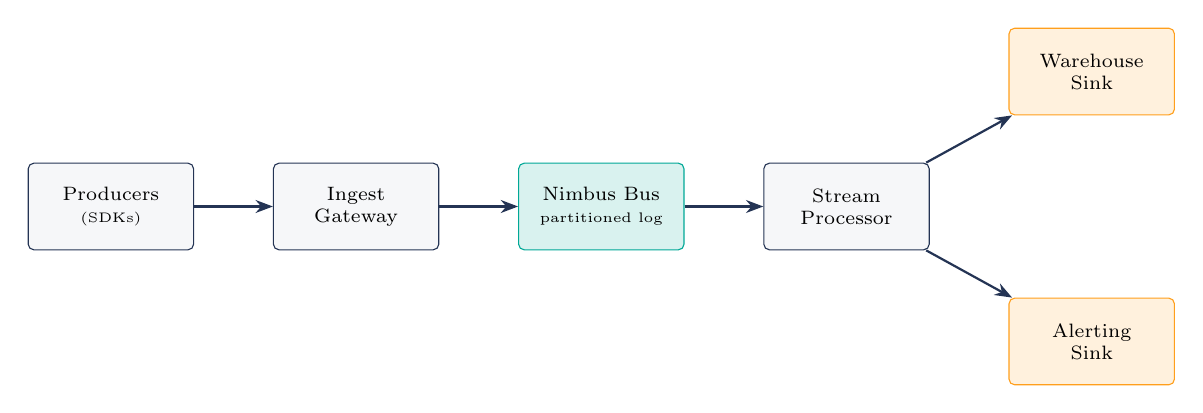
\begin{tikzpicture}[
      node distance=8mm and 10mm,
      box/.style={rectangle, draw=navySoft, fill=paperGray, rounded corners=2pt,
        minimum height=1.1cm, minimum width=2.1cm, align=center, font=\scriptsize},
      hub/.style={box, fill=tealAccent!15, draw=tealAccent},
      sink/.style={box, fill=amberAccent!15, draw=amberAccent},
      arr/.style={-{Stealth[length=2.2mm]}, thick, navySoft}
    ]
    \node[box] (prod) {Producers\\\tiny (SDKs)};
    \node[box, right=of prod] (gw) {Ingest\\Gateway};
    \node[hub, right=of gw] (bus) {Nimbus Bus\\\tiny partitioned log};
    \node[box, right=of bus] (proc) {Stream\\Processor};
    \node[sink, above right=6mm and 10mm of proc] (wh) {Warehouse\\Sink};
    \node[sink, below right=6mm and 10mm of proc] (al) {Alerting\\Sink};

    \draw[arr] (prod) -- (gw);
    \draw[arr] (gw) -- (bus);
    \draw[arr] (bus) -- (proc);
    \draw[arr] (proc) -- (wh);
    \draw[arr] (proc) -- (al);
  \end{tikzpicture}
  \vspace{0.6em}
  \begin{itemize}\small
    \item \textbf{Ingest Gateway} validates schema and stamps a monotonic offset
    \item \textbf{Nimbus Bus} is a partitioned append-only log (32 shards, 3x replicated)
    \item \textbf{Stream Processor} holds windowed state; scales independently of the bus
  \end{itemize}
\end{frame}

% ---------------------------------------------------------------------------
\begin{frame}{Data Flow Walkthrough}{Tracing one event from click to chart}
  \begin{columns}[T,onlytextwidth]
    \begin{column}{0.52\textwidth}
      \begin{enumerate}\small
        \item Client SDK emits event with idempotency key
        \item Gateway assigns partition via \texttt{hash(tenant\_id)}
        \item Bus appends to the shard's log, fsyncs to 2 of 3 replicas
        \item Processor consumes in order, updates windowed aggregates
        \item Sink writer commits offset only after downstream ack
      \end{enumerate}
    \end{column}
    \begin{column}{0.48\textwidth}
      \begin{table}
        \small
        \begin{tabular}{@{}lc@{}}
          \toprule
          \textbf{Stage} & \textbf{Budget} \\
          \midrule
          Gateway & 40 ms \\
          Bus append & 120 ms \\
          Processing & 300 ms \\
          Sink commit & 90 ms \\
          \bottomrule
        \end{tabular}
        \caption{Latency budget per stage}
      \end{table}
    \end{column}
  \end{columns}
\end{frame}

% ---------------------------------------------------------------------------
\sectiondivider{03 \textbullet\ Core Algorithm}{Adaptive partitioning \& consistent hashing}

% ---------------------------------------------------------------------------
\begin{frame}{Consistent Hashing Ring}{How we place shards without a full reshuffle}
  \begin{columns}[T,onlytextwidth]
    \begin{column}{0.48\textwidth}
      \begin{algorithm}[H]
        \DontPrintSemicolon
        \KwIn{event key $k$, ring $R$}
        \KwOut{owning shard $s$}
        $h \gets \text{hash}(k)$\;
        $s \gets$ first node in $R$ clockwise from $h$\;
        \If{$s$ is marked draining}{
          $s \gets$ next live node clockwise\;
        }
        \Return{$s$}\;
        \caption{Route(key, ring)}
      \end{algorithm}
    \end{column}
    \begin{column}{0.48\textwidth}
      \centering
      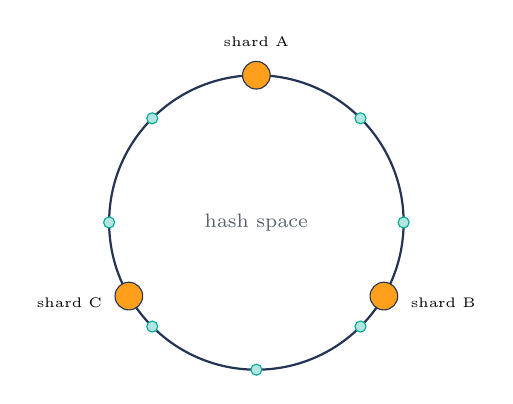
\begin{tikzpicture}[scale=0.85]
        \draw[navySoft, thick] (0,0) circle (2.2);
        \foreach \i in {0,...,7} {
          \node[circle, fill=tealAccent!30, draw=tealAccent, minimum size=4pt,
                inner sep=1pt] (n\i) at ({90-\i*45}:2.2) {};
        }
        \node[circle, fill=amberAccent, draw=navySoft, minimum size=10pt] at (90:2.2) {};
        \node[above=2pt] at (90:2.4) {\tiny shard A};
        \node[circle, fill=amberAccent, draw=navySoft, minimum size=10pt] at (-30:2.2) {};
        \node[right=2pt] at (-30:2.4) {\tiny shard B};
        \node[circle, fill=amberAccent, draw=navySoft, minimum size=10pt] at (210:2.2) {};
        \node[left=2pt] at (210:2.4) {\tiny shard C};
        \node at (0,0) {\scriptsize\color{inkGray} hash space};
      \end{tikzpicture}
    \end{column}
  \end{columns}
  \vspace{0.4em}
  {\small Only keys between the draining node and its clockwise neighbor move
  during a rebalance --- roughly \(1/N\) of all keys, not all of them.}
\end{frame}

% ---------------------------------------------------------------------------
\begin{frame}[fragile]{Live Coding: The Rebalance Handler}{What actually runs when a shard drains}
  \begin{lstlisting}[style=nimbus]
func (r *Ring) Rebalance(draining ShardID) error {
    next := r.NextLive(draining)
    keys := r.KeysOwnedBy(draining)

    for _, k := range keys {
        // Copy before repoint: never orphan a key mid-flight
        if err := r.Replicate(k, next); err != nil {
            return err // caller retries; ring stays consistent
        }
        r.Repoint(k, next)
    }
    r.MarkDrained(draining)
    return nil
}
  \end{lstlisting}
  \vspace{0.3em}
  {\small\color{inkGray} Replicate-then-repoint keeps the ring consistent even if
  the handler crashes mid-rebalance --- Nimbus Bus and the processor both read
  from the same ring version.}
\end{frame}

% ---------------------------------------------------------------------------
\begin{frame}{Complexity \& Guarantees}{What the algorithm buys us}
  \begin{table}
    \small
    \begin{tabular}{@{}lll@{}}
      \toprule
      \textbf{Operation} & \textbf{Cost} & \textbf{Guarantee} \\
      \midrule
      Route lookup & $O(\log N)$ & deterministic per ring version \\
      Shard add/remove & $O(K/N)$ keys move & no full reshuffle \\
      Rebalance & background, throttled & zero dropped events \\
      \bottomrule
    \end{tabular}
    \caption{$N$ = shard count, $K$ = total keys}
  \end{table}
  \vspace{0.6em}
  \begin{statbox}{Why not a simple modulo hash?}
    \texttt{shard = hash(key) \% N} reshuffles \emph{every} key whenever $N$
    changes. At 32 shards that meant re-copying \textbf{100\%} of state on every
    scale-out --- consistent hashing bounds that to about \textbf{3\%}.
  \end{statbox}
\end{frame}

% ---------------------------------------------------------------------------
\sectiondivider{04 \textbullet\ Results}{What changed in production}

% ---------------------------------------------------------------------------
\begin{frame}{Benchmarks: Before vs.\ After}{Measured over a 30-day production window}
  \begin{table}
    \small
    \begin{tabular}{@{}lrr@{}}
      \toprule
      \textbf{Metric} & \textbf{Legacy Batch} & \textbf{Nimbus Stream} \\
      \midrule
      p50 end-to-end latency & 6.2 min & 410 ms \\
      p99 end-to-end latency & 15.0 min & 1.8 s \\
      Max sustained throughput & 620K events/min & 5.1M events/min \\
      Sev-2 incidents / week & 3.6 & 0.2 \\
      \bottomrule
    \end{tabular}
    \caption{30-day rolling averages, production traffic}
  \end{table}
  \vspace{0.4em}
  {\small A 63\% reduction in on-call load came almost entirely from removing
  the shared batch window as a single point of contention.}
\end{frame}

% ---------------------------------------------------------------------------
\begin{frame}{Latency, Visually}{p50 / p99 side by side}
  \begin{columns}[T,onlytextwidth]
    \begin{column}{0.55\textwidth}
      \centering
      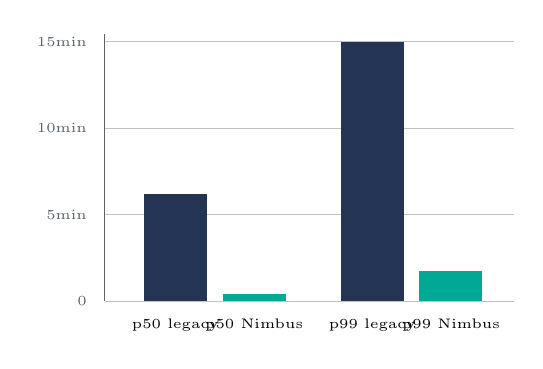
\begin{tikzpicture}[scale=1.0]
        \draw[inkGray] (0,0) -- (5.2,0);
        \draw[inkGray] (0,0) -- (0,3.4);
        \foreach \y/\lbl in {0/0, 1.1/5min, 2.2/10min, 3.3/15min}{
          \node[left, font=\tiny, color=inkGray] at (-0.1,\y) {\lbl};
          \draw[inkGray!40] (0,\y) -- (5.2,\y);
        }
        \fill[navySoft] (0.5,0) rectangle (1.3,1.36);
        \fill[tealAccent] (1.5,0) rectangle (2.3,0.09);
        \node[font=\tiny] at (0.9,-0.3) {p50 legacy};
        \node[font=\tiny] at (1.9,-0.3) {p50 Nimbus};
        \fill[navySoft] (3.0,0) rectangle (3.8,3.3);
        \fill[tealAccent] (4.0,0) rectangle (4.8,0.39);
        \node[font=\tiny] at (3.4,-0.3) {p99 legacy};
        \node[font=\tiny] at (4.4,-0.3) {p99 Nimbus};
      \end{tikzpicture}
    \end{column}
    \begin{column}{0.45\textwidth}
      \begin{itemize}\small
        \item p50 dropped from \textbf{6.2 min} to \textbf{410 ms}
        \item p99 dropped from \textbf{15.0 min} to \textbf{1.8 s}
        \item Tail latency is now dominated by processor window flush, not the bus
        \item Next target: p99 $<$ 1s by tightening window size
      \end{itemize}
    \end{column}
  \end{columns}
\end{frame}

% ---------------------------------------------------------------------------
\sectiondivider{05 \textbullet\ Lessons Learned}{What we'd do differently next time}

% ---------------------------------------------------------------------------
\begin{frame}{Lessons Learned}{Pros we'd repeat, cautions we'd heed}
  \begin{columns}[T,onlytextwidth]
    \begin{column}{0.5\textwidth}
      \begin{tcolorbox}[colback=tealAccent!8, colframe=tealAccent,
          title={\faThumbsUp\ Do Again}, coltitle=white,
          colbacktitle=navySoft, fonttitle=\bfseries]
        \begin{itemize}\small
          \item Replicate-then-repoint for every state migration
          \item Ship the ring as a versioned, immutable snapshot
          \item Load-test rebalancing \emph{before} the algorithm, not after
        \end{itemize}
      \end{tcolorbox}
    \end{column}
    \begin{column}{0.5\textwidth}
      \begin{tcolorbox}[colback=amberAccent!10, colframe=amberAccent,
          title={\faExclamationTriangle\ Watch For}, coltitle=white,
          colbacktitle=navySoft, fonttitle=\bfseries]
        \begin{itemize}\small
          \item Hot tenants can still overload a single shard
          \item Virtual nodes needed tuning --- too few caused skew
          \item Backpressure signals must reach producers, not just the bus
        \end{itemize}
      \end{tcolorbox}
    \end{column}
  \end{columns}
\end{frame}

% ---------------------------------------------------------------------------
\begin{frame}[plain]
  \begin{tikzpicture}[remember picture, overlay]
    \fill[navyDeep] (current page.south west) rectangle (current page.north east);
    \fill[tealAccent] ($(current page.north west)-(0,0.14)$) rectangle (current page.north east);
    \fill[amberAccent] (current page.south west) rectangle ($(current page.south east)+(0,0.14)$);
  \end{tikzpicture}
  \vfill
  \centering
  {\color{white}\Huge\bfseries Thank You\par}
  \vspace{0.5em}
  {\color{tealAccent}\large Questions, war stories, and disagreements welcome\par}
  \vspace{1.4em}
  {\color{white}\small \faEnvelope\ maya.chen@synapse.dev \hspace{1.2em} \faCode\ github.com/synapse/nimbus-stream\par}
  \vfill
\end{frame}

\end{document}
